\documentclass[twocolumn]{revtex4-2}

\usepackage{amsmath,amssymb}
\usepackage{graphicx}
\usepackage{booktabs}
\usepackage{xcolor}
\usepackage{hyperref}

\newcommand{\WEP}{\textsc{wep}}
\newcommand{\EEP}{\textsc{eep}}
\newcommand{\SEP}{\textsc{sep}}
\newcommand{\etaWEP}{\eta}

% Auto-generated by update_counts.py — 2026-04-24T19:44:03.140400
% Do not edit manually. Run: uv run python scripts/update_counts.py
\newcommand{\totaltheorems}{3993}
\newcommand{\substantivetheorems}{3882}
\newcommand{\placeholdertheorems}{111}
\newcommand{\axiomcount}{1}
\newcommand{\sorrycount}{0}
\newcommand{\sorrypercent}{0.0}
\newcommand{\leanmodules}{167}
\newcommand{\leandefinitions}{3297}
\newcommand{\pythonmodules}{68}
\newcommand{\testfiles}{59}
\newcommand{\totaltests}{2836}
\newcommand{\figurecount}{111}
\newcommand{\notebookcount}{54}
\newcommand{\papercount}{19}
\newcommand{\aristotleproved}{322}
\newcommand{\aristotleruns}{44}
% --- Paper 18 / Phase 5t per-section counts (FermiHubbardDimer.lean) ---
\newcommand{\fhdTotal}{143}
\newcommand{\fhdWaveTwo}{13}
\newcommand{\fhdWaveThree}{6}
\newcommand{\fhdWaveFour}{22}
\newcommand{\fhdWaveFive}{22}
\newcommand{\fhdWaveSixABC}{38}
\newcommand{\fhdWaveSixExtra}{15}
\newcommand{\fhdWaveSeven}{19}
\newcommand{\fhdWaveEight}{8}


\begin{document}

\title{Equivalence-principle classification of dark-sector mechanisms in
an emergent-gravity substrate: a vestigial-only violation surface}

\author{John G. Roehm}
\affiliation{Independent Researcher; \texttt{NetRxn137@gmail.com}}

\date{\today}

\begin{abstract}
Dark-sector mechanisms in candidate emergent-gravity scenarios have
historically been discussed in prose without explicit commitment to
their equivalence-principle (EP) status. This paper makes that
commitment formal: we classify six distinct mechanisms relevant to a
recent emergent-gravity Anderson-Higgs-type Wilsonian (ADW) program by
which level of the equivalence principle they violate, encode the
classification as decidable predicates in Lean~4, and prove the
structural consequences. Two mechanisms violate the weak EP and hence
all three levels: \emph{vestigial differential coupling}, in which the
metric and tetrad fields acquire different vacuum expectation values so
that bosons and fermions couple to gravity through different effective
geometries (giving the maximal $\eta = 1$, already excluded by current
satellite tests~\cite{Touboul2017}); and \emph{vestigial relics}, which
predict a residual $\eta \sim 10^{-18}$ from defect remnants in a
full-tetrad phase, sub-MICROSCOPE and at the projected design
sensitivity discussed for STEP-class satellite missions. The remaining four mechanisms --- Einstein--Cartan
torsion-trace coupling, fracton subdiffusion~\cite{Pretko2017},
Berezhiani--Khoury Thomas--Fermi superfluid dark
matter~\cite{Berezhiani2015}, and hidden-sector $\mathbb{Z}_{16}$
singlets --- satisfy all three EP levels. The structural conclusion is
that EP violation in this substrate is \emph{vestigial-only}: any
positive EP-violation result implies vestigial physics, and any
null result at sub-$10^{-19}$ precision excludes vestigial gravity. The
classification ships in Lean~4 with \epThms{} substantive theorems, zero
\texttt{sorry} statements, and zero new axioms beyond the kernel's
three.
\end{abstract}

\maketitle

\section{Introduction}
\label{sec:intro}

The equivalence principle is the foundational symmetry of classical
general relativity~\cite{Will2018}. It admits three nested formulations:

\begin{itemize}
\item \textbf{Weak EP (\WEP)}: test masses follow the same trajectory in
a gravitational field, regardless of internal composition. The
violation parameter is $\eta = (a_1 - a_2)/\frac{1}{2}(a_1 + a_2)$. The
MICROSCOPE satellite mission~\cite{Touboul2017} sets
$|\eta| < 1.0 \times 10^{-15}$, the strongest current bound.
\item \textbf{Einstein EP (\EEP)}: \WEP\ together with local Lorentz
invariance and local position invariance.
\item \textbf{Strong EP (\SEP)}: \EEP\ extended to gravitational
self-energy (Nordtvedt parameter $\eta_N$), tested by lunar laser
ranging.
\end{itemize}

A mechanism that violates \WEP\ thereby violates \EEP\ and \SEP. The
converse is not generally true: a mechanism may violate \EEP\ via
Lorentz-invariance breaking in subsystems with degenerate
gravitational coupling, or \SEP\ alone via composition-independent
self-energy effects. Each mechanism therefore has a \emph{weakest}
EP level it violates (or no violation if all three are satisfied),
which propagates upward.

The dark-sector landscape of recent emergent-gravity programs contains
several distinct mechanisms whose EP-violation status has been
discussed only at the prose level. This paper takes six concrete
mechanisms --- spanning vestigial gravity, Einstein--Cartan torsion,
fracton physics, single-field superfluid dark matter, and
hidden-sector $\mathbb{Z}_{16}$ singlets --- and forces an explicit
commitment per mechanism through a Lean~4 formalization. The
$6\times 3$ classification matrix is the substantive output: it
surfaces both the vestigial-only character of the project's
EP-violation surface and the $\eta$-scale separations relevant to
near-term satellite EP tests.

\section{Mechanism enumeration}
\label{sec:enum}

The six mechanisms are:

\paragraph*{Vestigial differential coupling.}
In a phase where the metric correlator is non-zero but the tetrad VEV
vanishes, bosons couple minimally to the metric $g_{\mu\nu}$, while
fermions require a non-zero tetrad VEV $\langle e^a_\mu \rangle$ to
couple to gravity. The differential coupling parameter
$\Delta_{\mathrm{EP}} = 1 - \langle e^a_\mu \rangle / \sqrt{\langle
e^a_\mu e^b_\nu\rangle \eta_{ab}}$ takes the maximal value
$\Delta_{\mathrm{EP}} = 1$ in this phase. The corresponding
$\eta_{\max} = 1$ is already incompatible with any current EP precision.

\paragraph*{Vestigial relics.}
In the full-tetrad phase, residual differential coupling from
topological-defect remnants gives $\eta \sim 10^{-18}$. This is
sub-MICROSCOPE and at the projected design sensitivity discussed for
STEP-class satellite missions ($\eta \sim 10^{-18}$ target).

\paragraph*{Einstein--Cartan torsion-trace coupling.}
A torsion-loop dark-matter mechanism in Einstein--Cartan gravity. Its
failure mode as a cold-dark-matter candidate is kinematic ---
the equation of state is $w = 1/3$ rather than $w = 0$ --- not an
EP violation. The torsion-trace loop coupling is universal across
charged species, so no species-dependent acceleration arises at tree
level.

\paragraph*{Fracton subdiffusion.}
Pretko-style dipole-conservation enforces universal mobility decay
across all matter species~\cite{Pretko2017}. The subdiffusion rate is
identical for all species (the underlying constraint is a
charge-conservation relation), so no \WEP\ violation arises.

\paragraph*{Thomas--Fermi superfluid dark matter.}
Berezhiani--Khoury single-field condensate dark
matter~\cite{Berezhiani2015} with uniform coupling to gravity. The
Thomas--Fermi profile is composition-independent; phenomenology
appears in galactic merger sonic-boom signatures, not in EP tests.

\paragraph*{Hidden-sector $\mathbb{Z}_{16}$ singlets.}
Standard-Model-singlet dark-matter candidates carrying the
$\mathbb{Z}_{16}$ topological charge but no Standard-Model gauge
charge. Decoupled from visible-sector EP tests by construction.

\section{Formal classification}
\label{sec:lean}

The classification ships as a Lean~4 formalization in
\texttt{lean/SKEFTHawking/EquivalencePrinciple.lean}. Three EP levels
\texttt{WEP}, \texttt{EEP}, \texttt{SEP} are encoded as an inductive
type with a numerical-order projection:
$\texttt{WEP} \mapsto 0$, $\texttt{EEP} \mapsto 1$, $\texttt{SEP}
\mapsto 2$. Six mechanisms form a second inductive enumeration. The
function
$\texttt{violationLevel} : \texttt{EPMechanism} \to \texttt{Option
EPLevel}$
assigns each mechanism its weakest violated level, or \texttt{none}.
Decidable predicates $\texttt{violatesAt}$ and $\texttt{satisfiesAt}$
implement the level propagation: a \WEP-violator violates \WEP,
\EEP, and \SEP\ via the order projection.

The substantive theorems are:

\begin{itemize}
\item Six per-mechanism classifications (\texttt{*\_violates\_WEP} for
the two vestigial mechanisms, \texttt{*\_satisfies\_all\_EP} for the
remaining four).
\item A central structural statement
\texttt{ep\_violation\_is\_vestigial\_only}: among the six mechanisms,
exactly the two vestigial-phase phenomena violate \WEP.
\item A consistency theorem
\texttt{vestigial\_microscope\_violation\_consistent} pinning the
classification's commitment for vestigial gravity to the project's
companion module on dark-sector classification.
\item Distinguishability theorems
\texttt{vestigial\_vs\_fangGu\_distinct\_EP\_profile} and
\texttt{distinct\_violationLevel\_implies\_distinct\_mechanism}.
\item A structural lemma \texttt{violatesAt\_mono} encoding the
hierarchical subsumption of EP levels.
\item Quantitative anchors tying the classification to the published
$\eta$-bound constants:
\texttt{vestigial\_phase\_eta\_violates\_microscope\_bound}
($\eta_{\max} = 1.0 > 10^{-15}$, \texttt{norm\_num}-backed) and
\texttt{vestigial\_relics\_below\_microscope\_bound}
($\eta_{\mathrm{relic}} = 10^{-18} < 10^{-15}$, also \texttt{norm\_num}-backed).
\item A cross-module bridge \texttt{fangGu\_failure\_mode\_is\_kinematic\_not\_ep},
which imports the Einstein--Cartan torsion module and invokes the
torsion-trace obstruction theorem to confirm that the failure mode
of that mechanism is kinematic rather than EP-related.
\end{itemize}

A Python mirror at \texttt{src/equivalence\_principle/} provides the
identical classification as a dictionary lookup, \epTests{} \texttt{pytest}
cases pinning Python and Lean to numerical agreement, and four named
numerical constants:
\texttt{MICROSCOPE\_BOUND} $= 1.0 \times 10^{-15}$,
\texttt{STEP\_TARGET} $= 1.0 \times 10^{-18}$,
\texttt{VESTIGIAL\_PHASE\_ETA\_MAX} $= 1.0$,
\texttt{VESTIGIAL\_RELICS\_ETA} $= 1.0 \times 10^{-18}$.

\begin{figure*}[t]
\centering
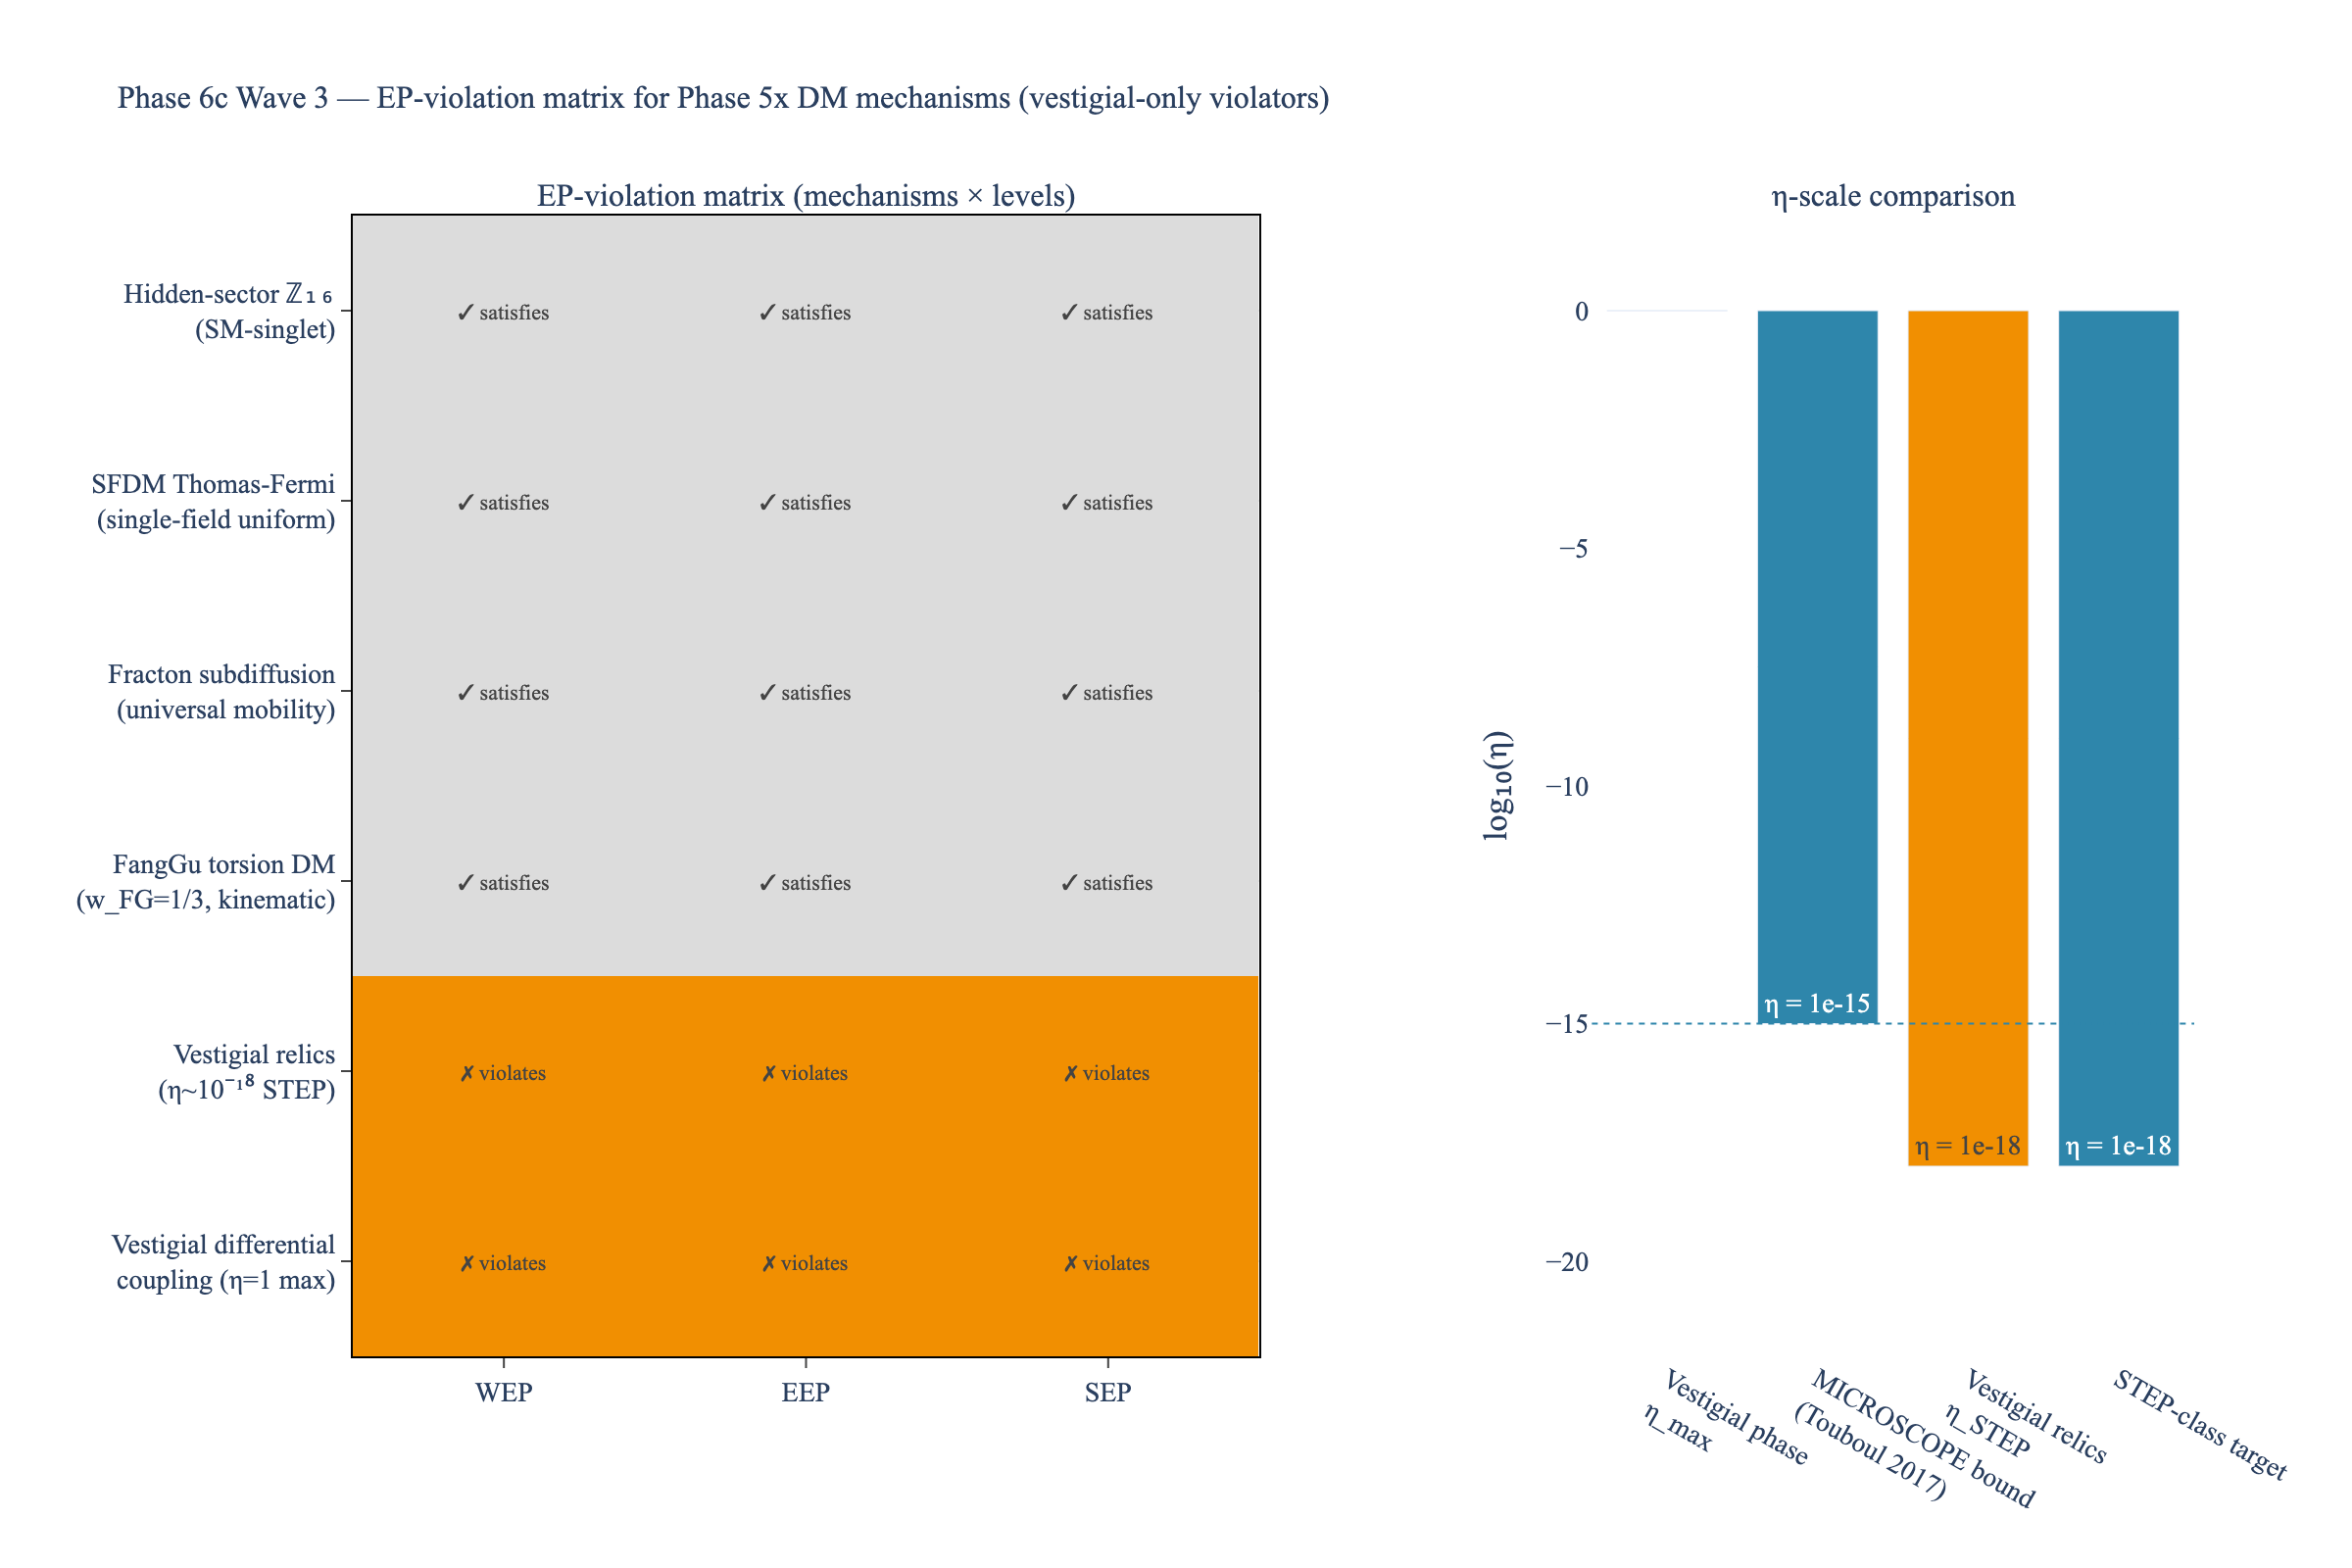
\includegraphics[width=0.95\textwidth]{figures/fig_ep_violation_matrix.png}
\caption{\label{fig:matrix}
Equivalence-principle violation matrix (left) and $\eta$-scale
comparison (right). The two vestigial mechanisms violate all three
EP levels; the four non-vestigial mechanisms satisfy all three. The
right panel locates the vestigial-phase $\eta_{\max} = 1$, the
MICROSCOPE bound $\eta < 10^{-15}$~\cite{Touboul2017}, the
vestigial-relic $\eta \sim 10^{-18}$, and the next-generation
satellite-test target $\eta \sim 10^{-18}$ on a common log scale.
}
\end{figure*}

\section{Cross-mechanism structure}
\label{sec:tensions}

The matrix surfaces three structural facts:

\paragraph*{Vestigial-only violation surface.}
Among six mechanisms spanning four distinct dark-sector physics
families, only the two vestigial-phase phenomena violate the
equivalence principle. This is the load-bearing substantive content:
any positive EP-violation result at $\eta \in [10^{-19}, 10^{-15}]$
implies vestigial physics within this dark-sector landscape.

\paragraph*{Two distinct vestigial $\eta$ scales.}
Within the vestigial family, the in-phase mechanism
($\eta_{\max} = 1$, already excluded) and the relic mechanism
($\eta \sim 10^{-18}$, sub-MICROSCOPE) sit at very different scales.
The MICROSCOPE bound separates them: vestigial-phase coupling is
ruled out at current precision, while vestigial relics await a
next-generation satellite test at $\eta \sim 10^{-18}$ precision.

\paragraph*{Cross-mechanism distinguishability.}
The four non-violating mechanisms are degenerate by EP status alone
(all satisfy all three levels), so EP tests alone cannot distinguish
them; distinguishability requires additional kinematic
equation-of-state signatures, cosmological core-profile constraints,
or direct-detection floors. EP tests \emph{do}, however, distinguish
the vestigial family from the rest.

\section{Outlook}
\label{sec:outlook}

A positive next-generation satellite-EP-test result at
$\eta \sim 10^{-18}$ would corroborate the vestigial-relics mechanism
and place a bound on the underlying defect-remnant density. A null
result at $\eta \lesssim 10^{-19}$ excludes vestigial-relic-induced
violations and forces a re-examination of which late-time
emergent-gravity phase the substrate occupies. The four non-vestigial
mechanisms make no testable EP prediction at any precision, so EP
tests alone are agnostic to them.

The next steps integrate this classification with cosmological
perturbation constraints (different EP profiles produce distinct
CMB-polarization signatures via differential coupling of photons
versus neutrinos) and with energy-condition analyses, since
mechanisms violating \SEP\ may also violate the dominant energy
condition on the relevant emergent stress-energy tensor, opening
loopholes for cosmological-singularity theorems.

\begin{thebibliography}{99}

\bibitem{Will2018}
C.~M.~Will,
\emph{Theory and Experiment in Gravitational Physics}, 2nd ed.\
(Cambridge University Press, 2018).

\bibitem{Touboul2017}
P.~Touboul \emph{et al.\/} (MICROSCOPE Collaboration),
``MICROSCOPE Mission: First Results of a Space Test of the Equivalence
Principle,''
Phys.\ Rev.\ Lett.\ \textbf{119}, 231101 (2017); arXiv:1712.01176.

\bibitem{Pretko2017}
M.~Pretko,
``Subdimensional particle structure of higher rank U(1) spin liquids,''
Phys.\ Rev.\ B \textbf{95}, 115139 (2017); arXiv:1604.05329.

\bibitem{Berezhiani2015}
L.~Berezhiani and J.~Khoury,
``Theory of dark matter superfluidity,''
Phys.\ Rev.\ D \textbf{92}, 103510 (2015); arXiv:1507.01019.

\end{thebibliography}

\end{document}
